\documentclass[conference]{IEEEtran}
\usepackage[utf8]{inputenc}
\usepackage[T1]{fontenc}
\usepackage{graphicx}
\usepackage{amsmath,amssymb}
\usepackage{booktabs}
\usepackage{url}
\usepackage{cite}
\IEEEoverridecommandlockouts

\begin{document}

\title{Verifiable-Reward Reinforcement Learning for\\ Post-OCR Transliteration of Kazakh Arabic Script\\ (T\"ote Jazu): A Feasibility Study}

\author{\IEEEauthorblockN{Yerali Agibayev}
\IEEEauthorblockA{Mathematical and Computational Science\\
Astana IT University\\
Astana, Kazakhstan\\
Email: yerali.agibayev@astanait.edu.kz}}

\maketitle

\begin{abstract}
T\"ote jazu, the Arabic-script orthography historically used to write Kazakh, is a
low-resource target for optical character recognition (OCR): no real-scan
benchmark exists, and the script's abjad nature creates systematic
many-to-one ambiguities that a purely visual model cannot resolve. We study
\emph{post-OCR transliteration}---mapping recognized Arabic-script characters to
Cyrillic---as a sequence-level task amenable to reinforcement learning with a
\emph{verifiable reward} (RLVR). We implement Group Relative Policy Optimization
(GRPO) with a deterministic edit-distance verifier, a KL penalty to a supervised
reference policy, and a short supervised warm-start, all trainable on CPU. On a
controlled synthetic testbed with linguistically motivated homographs, GRPO
reduces held-out character error rate (CER) of a lightly supervised base policy
from $0.605$ to $0.418$ ($31\%$ relative) using only the reward signal. We report
two strong baselines---a deterministic lookup table ($0.297$ CER) and a fully
supervised model ($0.277$ CER)---that GRPO does \emph{not} surpass on this
near-deterministic cipher, and we argue this is the expected outcome: RLVR's
value is concentrated in the ambiguous, noisy regime of real data, which we
identify as the next stage. This is a work-in-progress feasibility study; all
results are reproducible on CPU.
\end{abstract}

\begin{IEEEkeywords}
low-resource OCR, transliteration, reinforcement learning, verifiable reward,
GRPO, Kazakh, Arabic script
\end{IEEEkeywords}

\section{Introduction}
Kazakh has been written in three scripts over the last century; the Arabic-based
\emph{T\"ote jazu} remains in use among diaspora communities and in a large body
of pre-Cyrillic printed material. Digitizing this material requires OCR, but the
language is low-resource for this task in two compounding ways. First, to our
knowledge no public benchmark of \emph{real scanned} T\"ote jazu pages with
ground-truth transcriptions exists; prior Kazakh Arabic-script OCR work relies on
synthetic renderings. Second, the script is an \emph{abjad}: short vowels are
under-specified and several Cyrillic phonemes collapse onto a single Arabic-script
form, so that a visually perfect recognizer still faces an inherently ambiguous
inverse mapping back to Cyrillic.

This motivates treating transliteration as a distinct, learnable stage placed
\emph{after} the visual recognizer, and optimizing it for a sequence-level metric
(CER) rather than per-token likelihood. Reinforcement learning with a
verifiable reward (RLVR), in which a deterministic checker scores each sampled
output and no learned reward model is used, is a natural fit: the correctness of a
transliteration is checkable by string comparison, exactly as a math answer is
checkable in recent RLVR work~\cite{deepseekmath}.

This paper is a feasibility study with three contributions. (i) We give a
CPU-trainable RLVR pipeline for post-OCR transliteration based on
GRPO~\cite{deepseekmath} with an edit-distance verifier and a KL anchor to a
supervised reference. (ii) On a controlled synthetic testbed we show that GRPO
improves a lightly supervised base policy using the reward signal alone. (iii) We
report---rather than omit---two baselines that GRPO does not beat on this
testbed, and we explain why, delimiting precisely the regime in which RLVR is
expected to help and motivating the move to real data and a real OCR front-end.

\section{Related Work}
\textbf{Transformer OCR.} TrOCR~\cite{trocr} couples a vision-transformer encoder
with a text-transformer decoder and is the standard transfer-learning base for
low-resource scripts; the small variant is trainable on a single commodity GPU.
\textbf{Attention seq2seq.} Our transliteration policy is a GRU encoder--decoder
with dot-product attention~\cite{bahdanau}, which lets the decoder align output
character $i$ to the relevant input position and is what allows generalization
beyond memorized training words.
\textbf{Verifiable-reward RL.} Policy-gradient methods~\cite{reinforce,ppo} and
RL from human feedback~\cite{instructgpt} established the optimization machinery;
GRPO~\cite{deepseekmath} removes the value network by using group-relative
advantages and is the method we adopt. The defining feature of our setup is that
the reward is a \emph{deterministic verifier}, not a learned model.

\section{Method}
\subsection{Target pipeline}
The intended system has three stages: (1) synthetic image rendering of Cyrillic
Kazakh text through a script-conversion cipher and Arabic-script fonts, with
augmentation, to bootstrap training data; (2) a fine-tuned TrOCR recognizer
producing Arabic-script text; and (3) an RLVR \emph{post-correction /
transliteration} module producing Cyrillic. Stages (1)--(2) are future work
(Section~\ref{sec:limits}); this paper isolates and validates stage (3).

\subsection{Policy and supervised warm-start}
The policy $\pi_\theta$ is a bidirectional-GRU encoder and a GRU decoder with
dot-product attention (embedding $64$, hidden $128$). Pure RL from a random
initialization fails to leave the cold-start region, so we apply a short
supervised fine-tuning (SFT) warm-start with teacher forcing before RL, matching
the SFT$\rightarrow$RL recipe of modern alignment pipelines.

\subsection{GRPO with a verifiable reward}
For a source string we sample a group of $G=6$ candidate transliterations. Each
candidate $y$ is scored by a deterministic verifier
\begin{equation}
r(y, y^\star) = \bigl(1 - \mathrm{CER}(y, y^\star)\bigr) + 0.5\,\mathbb{1}[y = y^\star],
\end{equation}
where $\mathrm{CER}$ is the normalized Levenshtein distance and $y^\star$ is the
gold Cyrillic. Group-relative advantages
$\hat{A}_i = (r_i - \bar{r})/(\sigma_r + \varepsilon)$ replace a learned value
function~\cite{deepseekmath}. The objective combines the policy-gradient term with
a KL penalty to the frozen SFT reference $\pi_{\mathrm{ref}}$,
\begin{equation}
\mathcal{L} = -\,\mathbb{E}\!\left[\hat{A}\,\log \pi_\theta(y)\right]
\;+\; \beta\,\widehat{\mathrm{KL}}\!\left(\pi_\theta \,\|\, \pi_{\mathrm{ref}}\right),
\end{equation}
with $\beta = 0.04$ and the KL estimated on sampled tokens as
$\log\pi_\theta(y) - \log\pi_{\mathrm{ref}}(y)$. The KL term is essential: without
it, RL applied to an already-converged policy drifts and \emph{degrades} held-out
accuracy. Sampling temperature is annealed from $1.1$ to $0.6$. The entire
procedure runs on CPU.

\section{Experimental Setup}
\subsection{Controlled testbed}
Because no real aligned corpus is yet integrated, we evaluate on a synthetic
cipher that converts Cyrillic to a pseudo-Arabic alphabet. Crucially, the cipher
is \emph{not} a clean bijection: five linguistically motivated letter pairs
(front/back vowel and semivowel pairs that genuinely share one Arabic-script form,
e.g.\ the i/y and the close-vowel pairs) are mapped to a single glyph, so the
inverse task carries local, context-dependent ambiguity that mirrors real
T\"ote jazu. We stress that this is a \emph{machinery testbed}, not a linguistic
claim. The corpus is $420$ synthetic words, split $336/84$ into train/test;
source and target vocabularies are $29$ and $40$ symbols.

\subsection{Configurations}
We compare four systems on the same held-out set: (a) a deterministic
\emph{lookup table} mapping each Arabic glyph to its most frequent Cyrillic
pre-image in the training split; (b) \emph{SFT (light)}, $900$ warm-start steps,
used as the RL base policy; (c) \emph{SFT$\rightarrow$GRPO}, the light base
refined by $1500$ GRPO steps; and (d) \emph{SFT (full)}, $2500$ supervised steps.
During RL we monitor a $30$-word subset; the final table reports the full
$84$-word held-out set.

\section{Results}
\begin{table}[t]
\caption{Held-out results on the controlled testbed (full $84$-word test set).
Lower CER and higher exact-match are better.}
\label{tab:main}
\centering
\begin{tabular}{lcc}
\toprule
Method & Exact-match $\uparrow$ & CER $\downarrow$ \\
\midrule
Deterministic lookup table        & 0.143 & 0.297 \\
SFT (light, $900$) --- RL base     & 0.036 & 0.605 \\
\textbf{SFT$\rightarrow$GRPO (RLVR)} & \textbf{0.131} & \textbf{0.418} \\
SFT (full, $2500$)                 & 0.286 & 0.277 \\
\bottomrule
\end{tabular}
\end{table}

\begin{figure}[t]
\centering
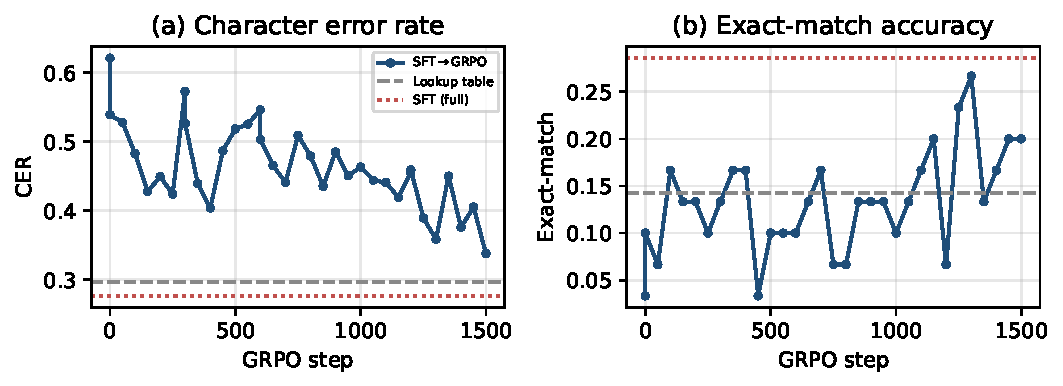
\includegraphics[width=\columnwidth]{curve.pdf}
\caption{GRPO learning curves on the held-out monitoring subset (n$=30$).
Dashed: deterministic lookup table. Dotted: fully supervised model. RLVR steadily
reduces CER over its supervised base but does not reach the stronger baselines on
this near-deterministic cipher.}
\label{fig:curve}
\end{figure}

Table~\ref{tab:main} and Fig.~\ref{fig:curve} report the outcome. Using only the
verifiable reward and a KL anchor, GRPO improves the light SFT base from $0.605$
to $0.418$ CER ($31\%$ relative) and from $0.036$ to $0.131$ exact-match. This
confirms that the RLVR machinery learns a real signal on CPU.

We deliberately report the two baselines GRPO does \emph{not} beat. The
deterministic lookup table reaches $0.297$ CER, and full supervised training
$0.277$. The narrow gap between these two is itself informative: even unlimited
supervision barely improves on a trivial table, because the synthetic words have
\emph{no morphological context} with which to disambiguate the shared-glyph
pairs. On a near-deterministic mapping with no exploitable context, a
likelihood-trained or rule-based model is the right tool, and RLVR's
exploration only adds variance. This is the expected boundary of the method, not
a contradiction of it: RLVR is predicted to help precisely where the target is
ambiguous and context-resolvable and where the input is noisy---neither of which
the present testbed provides.

\section{Limitations and Future Work}
\label{sec:limits}
The dominant limitation is that the corpus is a synthetic cipher rather than real
orthography, and there is as yet \emph{no OCR front-end}: the system transliterates
clean symbol strings, not recognizer output. Three concrete next stages follow
directly. First, replace the cipher with a real aligned corpus---an Arabic-script
/ Cyrillic parallel text---so that ambiguity and morphological context are
authentic; the RL code is unchanged and accepts such pairs directly. Second,
fine-tune a small TrOCR model on synthetically rendered pages (feasible on a free
cloud T4) to produce the realistic, \emph{error-bearing} input that makes
post-correction non-trivial. Third, evaluate RLVR specifically on the
disambiguation and OCR-error cases against the lookup-table and SFT baselines,
where the method is expected to show its advantage. We also plan an ablation of
the KL coefficient $\beta$ and group size $G$.

\section{Conclusion}
We presented a CPU-trainable, fully reproducible RLVR pipeline (GRPO with a
deterministic verifier and a KL-anchored reference) for post-OCR transliteration
of Kazakh Arabic script. On a controlled testbed the method demonstrably improves
a supervised base from the reward signal alone, while honest baselines locate the
regime---ambiguous, context-rich, noisy real data---in which it is expected to
pay off. The contribution is an end-to-end, verifiable scaffold and an honest map
of where the research must go next, rather than a premature state-of-the-art
claim on a toy task.

\begin{thebibliography}{1}
\bibitem{deepseekmath} Z. Shao \emph{et al.}, ``DeepSeekMath: Pushing the limits
of mathematical reasoning in open language models,'' \emph{arXiv:2402.03300},
2024.
\bibitem{trocr} M. Li \emph{et al.}, ``TrOCR: Transformer-based optical character
recognition with pre-trained models,'' in \emph{Proc. AAAI}, 2023.
\bibitem{bahdanau} D. Bahdanau, K. Cho, and Y. Bengio, ``Neural machine
translation by jointly learning to align and translate,'' in \emph{Proc. ICLR},
2015.
\bibitem{reinforce} R. J. Williams, ``Simple statistical gradient-following
algorithms for connectionist reinforcement learning,'' \emph{Machine Learning},
vol.~8, pp.~229--256, 1992.
\bibitem{ppo} J. Schulman \emph{et al.}, ``Proximal policy optimization
algorithms,'' \emph{arXiv:1707.06347}, 2017.
\bibitem{instructgpt} L. Ouyang \emph{et al.}, ``Training language models to
follow instructions with human feedback,'' in \emph{Proc. NeurIPS}, 2022.
\end{thebibliography}

\end{document}
